\section{Results: classification}
\label{sec:classification}

\subsection{Accuracy against target size}

Figure~\ref{fig:accuracy} shows accuracy against $k$ for all five data sets; Table~\ref{tab:k2} gives the values at $k = 2$. Accuracy rises with $k$ for every family. At $k = 2$, the Gaussian projection reaches \N{a:iris:2:gauss}\% on Iris against \N{af:iris}\% for all features, and \N{a:breast_cancer:2:gauss}\% on Breast Cancer against \N{af:breast_cancer}\%.

\begin{figure*}[t]
\centering
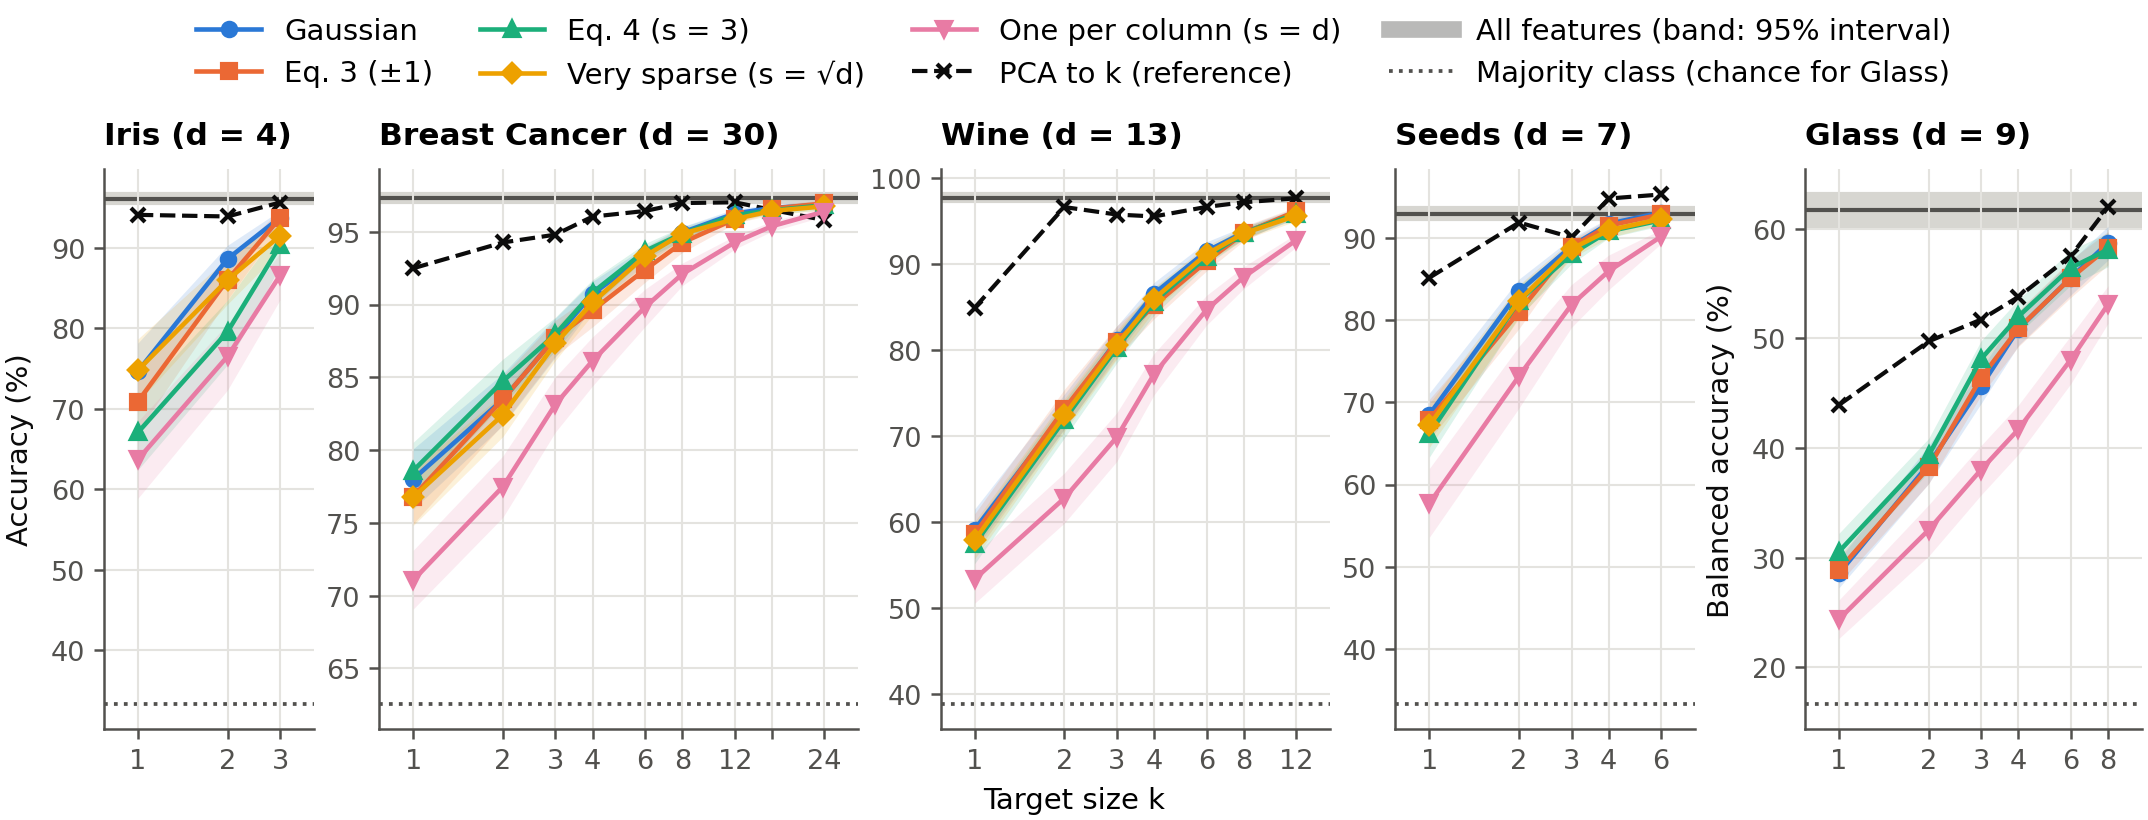
\includegraphics[width=\textwidth]{../study/figures/fig1_accuracy_vs_k_wide.png}
\caption{Test accuracy of the cross-validated model against target size $k$ for each data set (balanced accuracy for Glass), 100 draws each; bands are 95\% intervals. The gray line is all features, with its 95\% interval as a band; the dashed line is PCA to $k$; and the dotted line is the majority class (chance balanced accuracy for Glass). The horizontal axis is $k$ on a log scale. The very sparse family is not run on Glass.}
\label{fig:accuracy}
\end{figure*}

\begin{table}[t]
\caption{Test accuracy (\%) at $k = 2$, cross-validated model, mean over 100 draws (balanced accuracy for Glass). ``--'': not run. V. sparse: very sparse; 1/col.: one nonzero per column; All feat.: all features.}
\label{tab:k2}
\centering
\scriptsize
\setlength{\tabcolsep}{2.5pt}
\begin{tabular}{@{}lccccccc@{}}
\toprule
Data set & Gauss. & Eq. 3 & Eq. 4 & V. sparse & 1/col. & PCA & All feat. \\
\midrule
Iris & 88.6 & 86.0 & 79.6 & 86.0 & 76.5 & 93.9 & 96.1 \\
Breast Cancer & 83.5 & 83.5 & 84.7 & 82.4 & 77.5 & 94.3 & 97.3 \\
Wine & 72.8 & 73.1 & 71.9 & 72.4 & 62.8 & 96.6 & 97.7 \\
Seeds & 83.5 & 81.0 & 82.4 & 82.4 & 73.2 & 91.9 & 93.0 \\
Glass & 38.5 & 38.2 & 39.3 & -- & 32.5 & 49.7 & 61.7 \\
\bottomrule
\end{tabular}

\end{table}

\subsection{Sparse against dense}

Table~\ref{tab:comparisons} summarizes the \N{c:n_primary} primary comparisons, and Fig.~\ref{fig:paired} shows those against the Gaussian. After Holm's correction, \N{c:n_holm} differ, all of them losses. Of these, \N{c:opc_holm} are one nonzero per column against the Gaussian, and one is Eq.~4 on Iris at $k = 2$ (\N{pd:iris:2:eq4:gauss} points, 95\% interval [\N{pd:iris:2:eq4:gauss:lo}, \N{pd:iris:2:eq4:gauss:hi}], adjusted $p = \N{pd:iris:2:eq4:gauss:p}$; a Wilcoxon signed-rank test with the same Holm adjustment gives \N{wxh:iris:2:eq4:gauss}, so this result rests on the $t$-test). Eq.~3, Eq.~4 (outside Iris), and very sparse matrices show no loss against the Gaussian that survives the correction, and Eq.~4 against Eq.~3 does not differ either. Where the intervals are tight enough, equivalence within $\pm 2$ points holds: \N{z:equiv_total} of the \N{c:n_primary} comparisons are equivalent, mostly at the larger $k$ (for example, Breast Cancer for $k \ge 3$ with Eq.~4; Eq.~3 is also equivalent to the Gaussian on Breast Cancer at $k = 2$ and on Glass at $k = 1$), and \N{z:equiv_near} of them lie within 0.2 points of the margin. One comparison is in both the equivalence and the Holm-significant counts: one nonzero per column against the Gaussian on Breast Cancer at $k = 16$ (\N{pd:breast_cancer:16:opc:gauss} points, 95\% interval [\N{pd:breast_cancer:16:opc:gauss:lo}, \N{pd:breast_cancer:16:opc:gauss:hi}]) is equivalent and also significant after Holm's correction, a small but consistent loss. At small $k$, the intervals, up to \N{z:max_ci_side} points wide on each side, are often too wide to show equivalence.

\begin{figure*}[t]
\centering
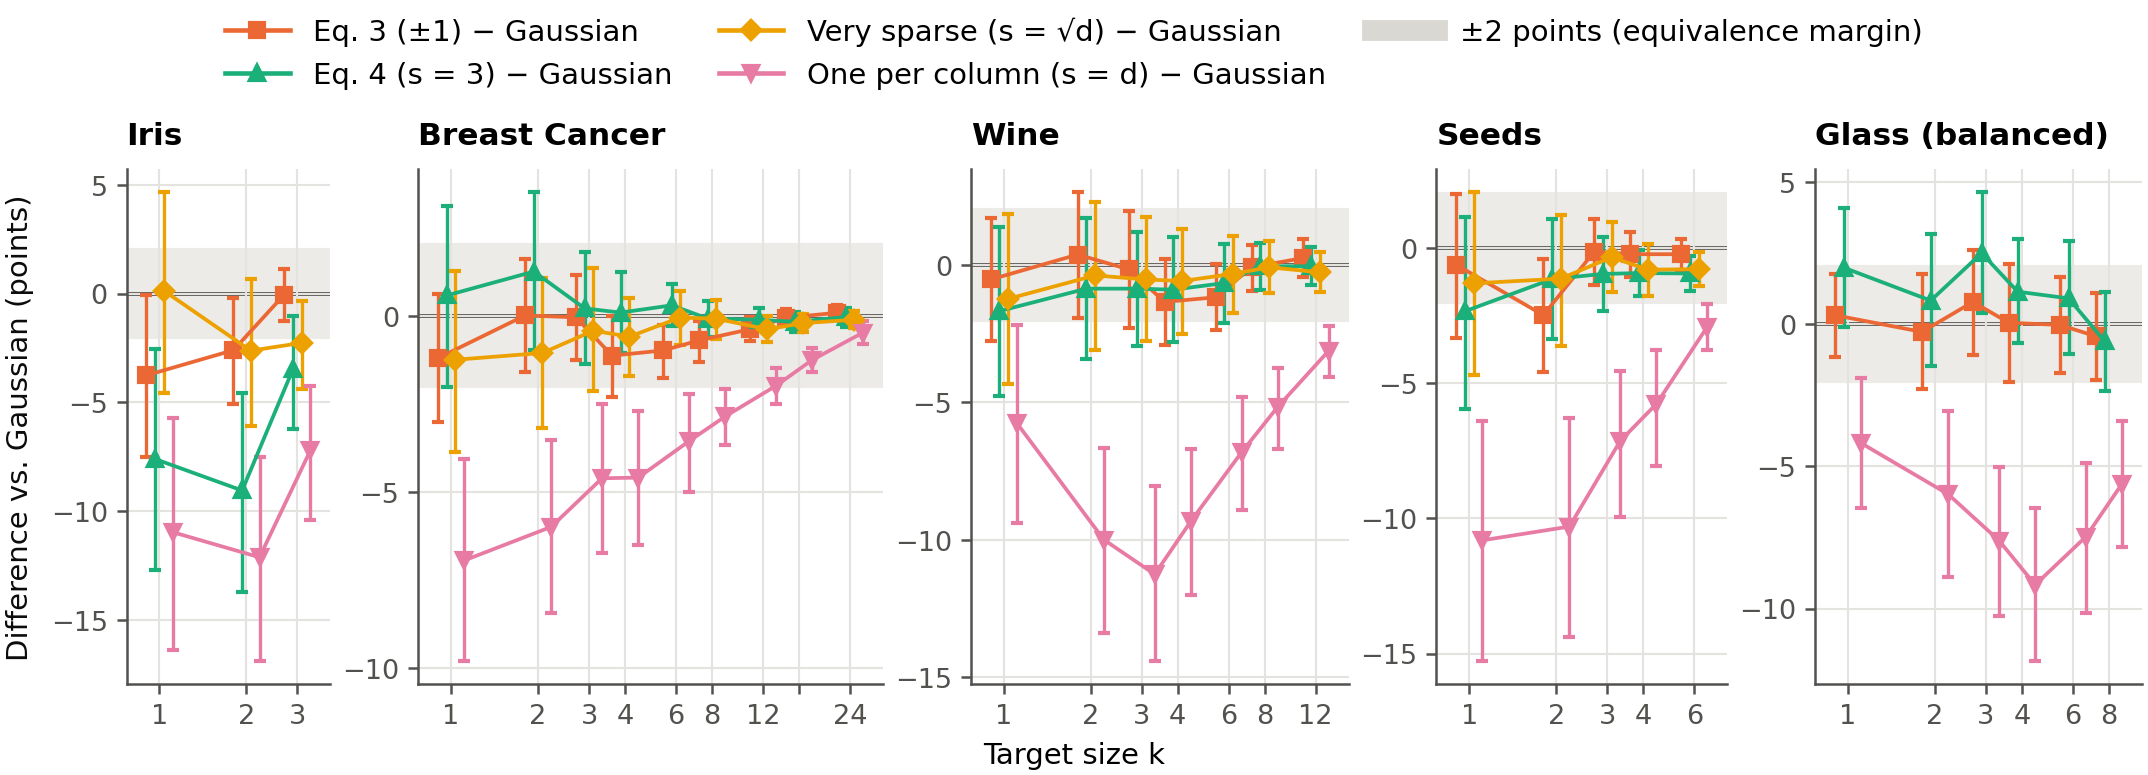
\includegraphics[width=\textwidth]{../study/figures/fig2_paired_difference_vs_gaussian_wide.png}
\caption{Paired difference from the Gaussian matrix in test accuracy of the cross-validated model, in points (balanced-accuracy points for Glass), against target size $k$: the mean over 100 draws with its 95\% interval. The shaded band is the $\pm 2$-point equivalence margin. The horizontal axis is $k$ on a log scale, and the four families are offset slightly in $k$ to make their intervals easier to tell apart.}
\label{fig:paired}
\end{figure*}

\begin{table*}[t]
\caption{The primary comparisons: cells, range of mean differences, comparisons whose 95\% interval lies inside $\pm 2$ points, comparisons whose interval excludes 0 (unadjusted), and comparisons significant after Holm's correction. Differences are in accuracy points (balanced-accuracy points for Glass).}
\label{tab:comparisons}
\centering
\footnotesize
\setlength{\tabcolsep}{4pt}
\begin{tabular}{@{}lccccc@{}}
\toprule
Comparison & Cells & Mean difference (points) & Within $\pm 2$ & Interval excludes 0 & After Holm \\
\midrule
Eq. 3 $-$ Gaussian & 30 & $-$3.8 to 0.8 & 16 & 6 & 0 \\
Eq. 4 $-$ Gaussian & 30 & $-$9.0 to 2.5 & 11 & 6 & 1 \\
Very sparse $-$ Gaussian & 24 & $-$2.6 to 0.1 & 12 & 3 & 0 \\
One per column $-$ Gaussian & 30 & $-$12.1 to $-$0.5 & 2 & 30 & 27 \\
Eq. 4 $-$ Eq. 3 & 30 & $-$6.4 to 1.8 & 11 & 3 & 0 \\
\bottomrule
\end{tabular}

\end{table*}

``No loss after Holm'' hides a small, consistent deficit. Very sparse minus Gaussian is negative in \N{c:vs_neg} of \N{c:vs_cells} cells, and Eq.~3 minus Gaussian in \N{c:eq3_neg} of \N{c:eq3_cells}. Pooled over draws, Eq.~3 trails the Gaussian by \N{mag:pool:eq3:gauss} points ($p = \N{pool:eq3:gauss:p}$; \N{mag:pool:eq3:gauss:noiris}, $p = \N{pool:eq3:gauss:noiris:p}$ without Iris), Eq.~4 by \N{mag:pool:eq4:gauss} ($p = \N{pool:eq4:gauss:p}$; \N{mag:pool:eq4:gauss:noiris}, $p = \N{pool:eq4:gauss:noiris:p}$ without Iris), and very sparse by \N{mag:pool:vs:gauss} ($p = \N{pool:vs:gauss:p}$; \N{mag:pool:vs:gauss:noiris}, $p = \N{pool:vs:gauss:noiris:p}$ without Iris). All of the pooled estimates are inside the $\pm 2$ margin, but with Iris, the 95\% interval of Eq.~4's deficit reaches \N{mag:poolci:eq4:gauss:lo} points, so the right statement is ``within about a point of dense'' outside Iris, not ``as good as dense.''

\subsection{Why Iris is the exception}

Iris has four features. Eq.~4 drops an average of \N{dz:iris:2:eq4:dropped_features_mean} of them at $k = 2$ (a feature is dropped when its row of the matrix is all zero), and leaves a column all zero in \N{z:iris_k2_zero_n} of the 100 draws, against \N{z:theory_zero_iris}\% in theory. Eq.~4 minus Gaussian is \N{pd:iris:1:eq4:gauss} points at $k = 1$, \N{pd:iris:2:eq4:gauss} at $k = 2$, and \N{pd:iris:3:eq4:gauss} at $k = 3$, each interval excluding zero and only $k = 2$ surviving Holm. The $k = 2$ loss comes from the draws with an all-zero column, about a third of them, and not from a typical draw. In the \N{z:iris_k2_zero_n} draws with an all-zero column, Eq.~4 trails the Gaussian by \N{mag:z:iris_k2_zero_mean} points, and by \N{mag:z:iris_k2_both_mean} when both columns are zero, so the projection is zero. In the other \N{z:iris_k2_full_n} draws, Eq.~4 is \N{z:iris_k2_full_mean} points ahead ($p = \N{z:iris_k2_full_p}$).

\subsection{One nonzero per column}

One nonzero per column trails the Gaussian in all \N{c:opc_cells} cells and after Holm in \N{c:opc_holm}, with losses from \N{z:opc_holm_min} to \N{z:opc_holm_max} points. At $k = 2$, it leaves a column all zero in \N{r0:z:opc_zero_min} to \N{r0:z:opc_zero_max} of the 100 draws on every data set. On Breast Cancer, the gap shrinks as $k$ grows (at $k = 24$: \N{mag:pd:breast_cancer:24:opc:gauss} points).

\subsection{Against PCA and all features}

PCA is a reference that sees the data. At $k = 2$, the Gaussian projection trails it by \N{pda:iris:2:gauss:pca} points on Iris, \N{pda:breast_cancer:2:gauss:pca} on Breast Cancer, \N{pda:wine:2:gauss:pca} on Wine, \N{pda:seeds:2:gauss:pca} on Seeds, and \N{pda:glass:2:gauss:pca} on Glass (balanced accuracy). Random projection comes within 2 points of all features only at larger $k$: from $k = 12$ on Breast Cancer, where $d = 30$ (\N{a:breast_cancer:12:gauss}\% against \N{af:breast_cancer}\%), at $k = 12$ on Wine, which has \N{z:d:wine} features and so no real reduction, and there in the means only (for the Gaussian, Eq.~3, and Eq.~4, the intervals reach \N{mag:pd:wine:12:eq3:full:lo} to \N{mag:pd:wine:12:gauss:full:lo} points below, and very sparse is \N{mag:pd:wine:12:vs:full} below), and at $k = 4$ to 6 on Seeds. It never does on Iris (best at $k = 3$: \N{pd:iris:3:gauss:full} points) or on Glass (best at $k = 8$: \N{pd:glass:8:gauss:full}). PCA is a reference with quirks: it standardizes its components, falls below the random projections on Breast Cancer at $k = 24$, and beats all features on Seeds at $k = 4$ and 6.

\subsection{Kernels}

On the Gaussian projection, the four tuned kernels' mean accuracies lie within \N{z:kern_spread_max} points of each other in every cell for Iris, Breast Cancer, Wine, and Seeds. On Glass, the linear kernel trails the best other kernel by \N{z:glass_trail_min} to \N{z:glass_trail_max} points of plain accuracy. Over all families and the two references, inner cross-validation picks the RBF kernel most often on Glass (\N{z:pick:glass:rbf}\% of classification rows) and the linear kernel most often on Iris (\N{z:pick:iris:linear}\%) and Seeds (\N{z:pick:seeds:linear}\%), where ties in inner accuracy are frequent and go to the linear kernel when it is tied for best; split evenly, the ties would put RBF first on both. Choosing among kernels on the test set, as the original report did, would have added about \N{z:test_optimism} points of optimism: the best of four kernels' test accuracies (plain accuracy for every data set) averages \N{z:best_test_acc}\% against \N{z:cv_test_acc}\% for the kernel chosen by cross-validation.
